\documentclass[12pt]{article}
\usepackage{amsmath}
\usepackage{graphicx,psfrag,epsf}
\usepackage{enumerate}
\usepackage{natbib}
\usepackage{url} % not crucial - just used below for the URL
\usepackage{subcaption}
\usepackage{booktabs}
\usepackage{hyperref}
\usepackage{float}
%\pdfminorversion=4
% NOTE: To produce blinded version, replace "0" with "1" below.
\newcommand{\blind}{0}

\usepackage{amsfonts}
\usepackage{wrapfig}
\newcommand{\Prob}{P}
\newcommand{\Expect}{\mathbb{E}}
\newcommand{\Reals}{\mathbb{R}}
\newcommand{\KL}{\textrm{KL}}

% DON'T change margins - should be 1 inch all around.
\addtolength{\oddsidemargin}{-.5in}%
\addtolength{\evensidemargin}{-.5in}%
\addtolength{\textwidth}{1in}%
\addtolength{\textheight}{-.3in}%
\addtolength{\topmargin}{-.8in}%

\DeclareMathOperator*{\argmax}{arg\,max}
\DeclareMathOperator*{\argmin}{arg\,min}

\usepackage{soul}
\usepackage[disable]{todonotes}
\newcommand{\jeff}[2][]{\todo[inline,color=blue!30, #1]{#2 \mbox{--Jeff}}}
\newcommand{\bryan}[2][]{\todo[inline,color=green!30, #1]{#2 \mbox{--Bryan}}}
 

\begin{document}

%\bibliographystyle{natbib}

\def\spacingset#1{\renewcommand{\baselinestretch}%
{#1}\small\normalsize} \spacingset{1}


%%%%%%%%%%%%%%%%%%%%%%%%%%%%%%%%%%%%%%%%%%%%%%%%%%%%%%%%%%%%%%%%%%%%%%%%%%%%%%

\if1\blind
{
  \title{\bf Reweighted Wake-Sleep for Deblending Crowded Starfields}
  \author{Author 1\thanks{
    The authors gratefully acknowledge \textit{please remember to list all relevant funding sources in the unblinded version}}\hspace{.2cm}\\
    Department of YYY, University of XXX\\
    and \\
    Author 2 \\
    Department of ZZZ, University of WWW}
  \maketitle
} \fi

\if0\blind
{
  \bigskip
  \bigskip
  \bigskip
  \begin{center}
    {\LARGE\bf Reweighted Wake-Sleep for Deblending Crowded Starfields}
\end{center}
  \medskip
} \fi

\bigskip
\begin{abstract}
The text of your abstract. 200 or fewer words.
\end{abstract}

\noindent%
{\it Keywords:}  3 to 6 keywords, that do not appear in the title
\vfill

\newpage
\spacingset{1.45} % DON'T change the spacing!
\section{Introduction}
\label{sec:intro}
Astronomical surveys play an important role in developing scientific knowledge of the universe.
The raw data in the form of telescope images
are often condensed into catalogs of light sources. 
Catalogs record light sources as stars, galaxies, or other objects; they also list physical parameters such as flux, color, and morphology. Astronomers employ catalogs for myriad downstream analyses. For example, the Argonaut map used the fluxes and colors of stars to construct the 3D distribution of interstellar dust~\cite{Green_2019_argonaut}. Spatial distributions of galaxies have been used to 
validate theoretical models of dark matter and dark energy~\cite{Eisenstein_2005_darkmatter}. 

\jeff{
Some of the text below may be useful in the introduction.
I haven't published it elsewhere, so feel free to include any parts verbatim if they are useful.

Light source separation, also known as ``deblending'', is the task of identifying and characterizing each imaged light source.
It is the starting point for most analysis of astronomical images---one of the few sources of data about the Universe beyond our solar system.

Light source separation is challenging for several reasons.
First, it is an ``unsupervised'' machine learning problem with a sample size of one: there is not labeled data with known ground truth, and there is only one night sky, which is imaged many times.
Second, many stars and galaxies too faint to be unambiguously resolved. For these light sources, providing calibrated uncertainty estimates of our predictions is as important as making accurate predictions.
Third, many stars and galaxies overlap with other light sources---as many as 68\% of galaxies are expected to overlap with others in upcoming LSST survey.
As telescopes improve, even more galaxies will appear to overlap.
Fourth, the scale of the data is immense by any standard. The upcoming LSST survey, scheduled to begin data collection in 2022, is expected to produce 50 petabytes of astronomical images over its lifetime---approximately 15 terabytes nightly.
}
\jeff{You might consider putting an image of a crowded starfield on the first or second page; without an image readers may not fully understand what we're talking about}

We focus on applications where all sources are well-modeled as points without spatial extent. Estimation of location, fluxes, and color is the primary goal.
Point sources are good models for surveys where the primary objects studied are stars, such as DECam~\cite{Schlafly_2018_DECam}, which imaged the center of our own Milky Way. Point source models are also used for surveys like WISE~\cite{Wright_2010_WISESurvey} whose telescope's resolution and the density of light sources did not allow for differentiation between stars and galaxies. 

In this paper, we apply our method to images of the globular cluster M2 from the Sloan Digital Sky Survey (SDSS). 
Understanding these starfields is of scientific interest per se. The distribution
of colors and fluxes in crowded starfields 
can be used to estimate the age 
of the starfield, which in turn lower bounds the 
age of the universe~\cite{Isochrome_fitting}. 

For all the aforementioned applications, a key challenge
in catalog construction is the {\itshape blending} of light sources: in crowded fields, sources are no longer well-separated, and peak intensities may correspond to multiple sources. An algorithm producing a catalog should be able to reliably {\itshape deblend} the peak intensity, that is, distinguish whether the peak corresponds to one light source or 
multiple light sources. When the two cases are nearly unidentifiable from the data, the algorithm should 
report calibrated uncertainties. As telescopes peer deeper into space, most images from future surveys will be in the crowded field regime. 
For example, \cite{Bosch_2017_LSST} estimates that in the Large Synoptic Survey Telescope (LSST), 68\% of the light sources will be blended. Therefore, developing a method to produce reliable catalogs even in cases of significant source blending will be important for advancing astronomical research. 

\subsection{From algorithmic pipelines to probabilistic cataloging}

Traditionally, most cataloging has been done using purely algorithmic pipelines, with steps involving locating the the brightest peaks, estimating fluxes, subtracting out the estimated light source, and repeating. Most of these pipelines are not designed for crowded starfields. 
In fact, the default SDSS cataloging pipeline, called PHOTO~\cite{lupton2001sdss}, failed to 
produce a catalog on 
the globular cluster M2~\cite{Portillo_2017}. 
Not only do these pipelines fail in the crowded field
regime, but they also do not produce statistically calibrated error estimates that propagate 
uncertainties accumulating in each step of the pipeline. 

Previous work in \cite{Brewer_2013, Portillo_2017, Feder_2019}
propose {\itshape probabilistic} cataloging.
They propose a statistical model consisting of a likelihood for the observed image and a prior distribution on possible catalogs. Instead of deriving a single catalog, they produce a Bayesian posterior distribution on the space of all possible catalogs. 
Each sample from the posterior is a catalog; that is, posterior samples are tables, potentially of varying length, consisting of stellar locations, fluxes, and colors. Uncertainties are fully quantified by the posterior distribution. For example, in an image with an ambiguously blended bright peak, some catalogs drawn from the posterior would contain multiple dim sources while others would contain one bright source. The relative weight the posterior distribution places on one explanation over another represents the statistical confidence in that explanation. Moreover, a distribution over the space of all catalogs induces a distribution on any estimate derived from a catalog. Therefore, uncertainties can be fully propagated to downstream analyses.  

In previous work on probabilistic cataloging, the posterior was computed using
Markov chain Monte Carlo (MCMC).
\cite{Portillo_2017, Feder_2019} refer to their method as PCAT, short for ``Probabilistic CATaloging."\footnote{
we will 
use ``probabilistic cataloging'' to refer to any method that produces a Bayesian posterior over possible catalogs; ``PCAT" refers specifically the the MCMC procedure in~\cite{Portillo_2017, Feder_2019}. }
However, the computational cost of MCMC is prohibitive for
large-scale astronomical surveys. PCAT required 30 minutes to process a $100\times 100$ pixel subimage of the globular cluster M2~\cite{Feder_2019}, roughly a $0.3\times0.3$ arcsecond patch of the sky.
For comparison, in one night SDSS scans a region of size on the order of $10 \times 1000$ arcminutes. Extrapolating the reported 30min runtime, PCAT would take about two months to process one night's data collection.
Future surveys will only get larger. LSST will collect at least 10 terabytes of data nightly, and hundreds of terabytes in total~\cite{LSST_about}. A crucial task is to develop inference methods that scale to these larger astronomical surveys. 

\subsection{Variational inference and neural networks}
As an alternative to MCMC, we construct an approximate posterior using variational inference~\cite{Blei_2017_vi_review,Jordan_intro_vi, Wainwrite_graph_models_vi}.
With variational inference (VI), we propose a family of distributions and use numerical optimization to find the distribution 
in the proposed family that is closest 
in KL divergence to the exact posterior. 
With a sufficiently constrained family of distributions, the VI optimization problem can be orders of magnitude faster than MCMC. 

We are not the first to propose a VI procedure
that scales Bayesian inference to the terabytes of data collected by astronomical surveys. 
\cite{regier2019_celeste} also employed 
VI, and with the help of a 650,000 core supercomputer, it constructed a catalog of the entire Sloan Digital Sky Survey based on Bayesian inference. 

However, one limitation of \cite{regier2019_celeste} is that the number of light sources in a given image is treated as known and fixed in their statistical model; thus, it had to be set by a preprocessing routine. In this work, the number of sources is assumed to be unknown and modeled as a latent variable. 
This results in a transdimensional latent variable space 
since the posterior is defined over the set of all catalogs, and the number of sources in a catalog is unknown and random.
Previous work on probabilistic cataloging employed reversible jump MCMC~\cite{Green95reversiblejump} to sample transdimensional catalogs. In RJ-MCMC, auxiliary variables are added to encode the ``birth" of new sources 
or the ``death" of existing sources in the Markov chain. Our challenge in VI is to construct a family of distributions on this transdimensional space. Section~\ref{sec:var_distr} discusses our construction: we define the variational distribution over catalogs of all possible size; that is, we define a distribution on a triangular array of latent locations and fluxes, and we map this to a distribution 
on the space of all catalogs.

Secondly, in \cite{regier2019_celeste}, numerical optimization had to be re-run for every new collection of images. 
In contrast, we employ {\itshape amortized} variational inference, where a neural network is trained to map input images to a variational distribution. After a one-time cost to train the neural network, inference 
on a new image requires just a single forward pass. In our 
architecture, detailed in Section~\ref{sec:nn_archetecture}, the forward pass on 
a $100 \times 100$ pixel subimage of M2 takes $\approx 0.2$ seconds (compare with 30min with MCMC). Moreover, neural networks can evaluate batches of images in parallel on a GPU. This amortization is advantageous for scaling up inference to large astronomical surveys.
\jeff{The most serious limitations of~\cite{regier2019_celeste} are that 1) the number of light sources is set by a preprocessing routine and fixed, 2) the variational distribution for some random variables is a point mass, including location.
This paper fixes both problems by using stochastic optimization, whereas~\cite{regier2019_celeste} used deterministic optimization.
Stochastic optimization is in general slower than deterministic optimization, but in this paper we get a speedup by using amortized inference.
In addition to greater speed, amortized inference may be better at nonconvex optimization: by learning a policy from many examples we learn a policy for avoiding shallow local minima. No carefully hand-tuned initialization scheme is needed.
}
\bryan{Wait, could you explain a bit more about how stochastic optimization helps us avoid (1) and (2)? 
I agree that these two issues should be mentioned, since
simply saying "we are faster" than this other VI procedure might not be enough motivation for this work. }

Neural networks have seen great success on image classification tasks~\cite{imagenet2015}, and we leverage their predictive power and computational efficiency for our problem of detecting and deblending stars. While in most applications of deep learning to image data, the neural network output is a ``label" -- whether the image is classified to be of one object or another -- in our work, we interpret the neural network output as specifying an approximate Bayesian posterior in the context of a well-defined statistical model. 

\subsection{The wake-sleep algorithm}

One limitation of neural networks is the large amount of data often needed for training.
In astronomy, knowledge of the physical system sometimes give rise to reasonably realistic simulators for data. For example, \cite{Lanusse_2017_cmudeeplens} used simulators to train neural networks to detect Einstein rings, 
a rare object found in astronomical surveys and used to study dark matter; the neural network in \cite{Hezaveh_2017_nn_lensing_nature} also returned
morphological parameters for each Einstein ring. 
In both cases, because the training data was generated from a simulator, the ground truth labels (ring exists or not; the ring morphology) are known. The network is trained in a supervised fashion. Using realistic simulated data is especially useful because the network can be trained on essentially unlimited data -- the bottleneck is the limit on computational resources, not the availability of training data. 

In our work, we also make use of simulated data for training. However, we introduce the simulated data in the context of a statistical model. In addition, we train the network to provide an approximate Bayesian posterior as discussed in the previous subsection, rather than a simple class label. 

To do so, we employ the wake-sleep algorithm~\cite{Hinton1995wake_sleep}. 
In the sleep-phase of the algorithm, we generate images and their corresponding catalogs from the statistical model. The loss function 
in the sleep phase encourages the neural network
to map simulated images to distributions that place probability mass on the their corresponding catalogs.
Minimizing this loss is equivalent to minimizing the ``forward" KL divergence between the variational distribution $q$ and the true posterior $p$, defined as $p$-weighted average difference between $\log p$ and $\log q$. 

This is not the same KL divergence used in traditional variational inference. In traditional variational inference, the loss function is the ``reverse" KL, where the difference between $\log p$ and $\log q$ is weighted by $q$. We will show empirically in our application that optimizing the forward KL produces more reliable approximate posteriors than optimizing the more traditional reverse KL. In particular, by taking advantage of large amounts ``labeled" data -- the simulated images and their corresponding catalogs -- the optimization is able to avoid shallow local minima where the approximate posterior returned by the neural network is far in KL from the true posterior. 

However, because the sleep phase makes use of simulated data from the statistical model, the statistical model should match as close as possible to the real data generating process. 
Thus, in the ``wake" phase, the variational distribution is fixed, and model paramters are estimated. This is equivalent to the M-step in variational EM~\cite{Jordan_intro_vi, neal2000varem, Beal2002varem}. In this application, the wake-phase is used to estimate the point spread function and the sky background in telescope images. 

In summary, we take advantage of the flexibility of neural networks to construct a mapping from input data to an approximate Bayesian posterior. To train the neural network, we employ simulated data in a statistically principled way. Because both the image and the catalog are known in the simulated data, we are able to recover a mapping that avoids shallow local minima in a difficult nonconvex optimization problem. Model parameters such as the point spread function are also tuned. 

We call our method to produce probabilistic catalogs {\itshape Starnet.}
In Section 5, we compare
the catalog obtained from Starnet with the MCMC-based cataloger PCAT;
we also compare with traditional cataloging approaches.

% However, in addition to greater speed, amortized inference may be better at nonconvex optimization: by learning a policy from many examples we learn a policy for avoiding shallow local minima. 



% In particular, the usual stochastic gradients of the reverse KL 
% were too high-variance to be used in in our application; 
% in contrast, low-variance stochastic gradients of the forward KL are computationally cheap to compute. 


% low-variance stochastic gradients of the forward KL are much cheaper to compute than stochastic gradients of the reverse KL. Moreover, we hypothesize that amortized inference may be better at nonconvex optimization: by learning a policy from many examples we learn a policy for avoiding shallow local minima. 






% The neural network outputs are not simply ``labels" for the input image 






% In traditional variational inference, the divergence between 
% the variational posterior $q$ and the true posterior $p$ is 
% measured by the ``reverse" KL divergence, defined as the 
% $q$-weighted average difference between $\log q$ and $\log p$. In other words, the reverse KL divergence
% is defined by an expectation with integrating distribution $q$. 

% In simple models, for example when $p$ and $q$ are appropriate classes of exponential families, 
% the expectation over $q$ can be written explicitly as a function of the parameters of $q$. Therefore, the minimizer of the KL can be solved either in closed form or by employing deterministic optimization~\cite{Blei_2017_vi_review}. 

% In our setting of amortized variational inference, the parameters of $q$ are neural network weights. When analytic expectations are unavailable, as in our case, 
% sampling methods have been employed in conjunction with modern auto-differentiation tools to compute stochastic gradients. Optimization is done with stochastic gradient descent. Examples include black-box variational inference (BBVI)~\cite{ranganath2013black} 
% and automatic-differentiation variational inference (ADVI)~\cite{kucukelbir2016automatic}. The latter 
% is closely related to the reparameterization trick \cite{kingma2013autoencoding, rezende2014stochastic} proposed to train deep generative models using the KL objective. 
% These approaches all sample latent variables from $q$ and produce an unbiased estimate 
% for the gradient of the KL. 

% However, the reparameterization trick does not apply when any latent variables are discrete, in our case, the number of stars. The REINFORCE estimator~\cite{Williams1992reinforce}, which BBVI adapts, produces an unbiased stochastic gradient for both continuous and discrete latent variables. However, the REINFORCE estimator often suffers from high variance in practice, and so the resulting stochastic optimization is slow. 

% The key difficulty is that the the objective function is 
% an expectation with integrating distribution on $q$, the  distribution to be optimized. To avoid this issue, the {\itshape wake-sleep} algorithm considers the ``forward" KL divergence, defined as the
% $p$-weighted average difference between $\log p$ and $\log q$;  in other words, the expectation is taken over $p$. To make the forward KL divergence tractable, a second average is taken over possible data. In other words, the neural network is trained so that {\itshape on average over possible input images $x$}, the 
% variational distribution returned by the neural network is close to the true posterior in forward KL divergence. 

% Low-variance stochastic gradients are easy to compute using the wake-sleep algorithm, and we show that these low-variance gradients result in faster optimization than using the REINFORCE gradient estimator. 
% However, in addition to greater speed, amortized inference may be better at nonconvex optimization: by learning a policy from many examples we learn a policy for avoiding shallow local minima. 



% In simple models, for example when both $p$ and $q$ are related exponential families, the expectation can be written explicitly as a function of the parameters of $q$~\cite{Blei_2017_vi_review}. Therefore, the KL can be minimized either in closed form, or by using deterministic optimization. However, in our case, the parameters of $q$ are neural network weights. In this setting, ~\cite{rezende2014stochastic,kingma2013autoencoding} propose 
% stochastic optimization, where an unbiased gradient of the KL divergence is computed from samples of $q$. 





% One limitation of neural networks is the large amount of data needed for training.
% In astronomy, knowledge of the physical system  often give rise to reasonably realistic simulators for data. For example, simulators were used in \cite{Lanusse_2017_cmudeeplens} trained neural networks to detect Einstein rings, 
% a rare object found in astronomical surveys and used to study dark matter; the neural network in \cite{Hezaveh_2017_nn_lensing_nature} also returned
% morphological parameters for each Einstein ring. 
% In both cases, because the training data was generated from a simulator, the ground truth labels (ring exists or not; the ring morphology) are known. The network is trained in a supervised fashion. Using simulated data is especially useful because the network can be trained on essentially unlimited data -- the bottleneck is the limit on computational resources, not the availability of training data. 

% In our work, we also make use of simulated data to train our neural network. However, we introduce the simulated data in the context of a statistical model. We do so using the wake-sleep algorithm~\cite{Hinton1995wake_sleep}. 
% The neural network outputs are not simply ``labels" for the input image; rather, we are able to interpret the output as specifying an approximate Bayesian posterior in the context of a well-defined statistical model. 

% In summary, we leverage the predictive power and computational efficiency of neural networks to do 
% inference in the framework of a statistical model. 
% We also employ simulated data in our training procedure in a statistically principled way. In Section~\ref{sec:results}, we compare the catalog obtained from our variational posterior with the catalog derived from MCMC; we also compare with traditional cataloging approaches.  

% detect Einstein rings; \cite{Hezaveh_2017_nn_lensing_nature} used
% neural networks to infer morphological characteristics of the Einstein rings; 
% in the context of deblending, 
% \cite{Reiman_2019_gans_deblend} used 
% GANS to separate two overlapping galaxies. 

% Several factors contribute to the success of neural networks. Firstly, neural networks are computationally efficient; multiple images can be easily evaluated in parallel on a GPU.
% Secondly, a well-trained neural network is able to generalize beyond the data on which is was trained. This combined with computational efficiency is extremely beneficial for sky surveys: after training a neural network on a subset of the survey, the remaining images in the survey can be evaluated quickly in batches using only forward-passes through the network. 

% In this paper, we combine the flexibility of neural networks with a formal statistical model. This enables the neural network output to be interpreted in a statistically principled way: the output of our neural network will be a distribution that approximates the Bayesian posterior.

% Secondly, we train the neural network using {\itshape wake-sleep} training. This allows our neural network to be trained using unlimited simulated data. Using simulated data to train neural networks is common practice is astronomy (see for example~\cite{Lanusse_2017_cmudeeplens, huang2019finding}). However, we also make the connection with a formal statistical model 
% and introduce the simulated data in a principled way. TODO: yikes ... this paragraph is terrible and needs work. 

% In Section~\ref{sec:gen_model} we introduce 
% the generative model. Section~\ref{sec:var_inference} details the variational distribution and discuss training of the neural network. Section~\ref{sec:related_work} makes connections with previous cataloging software. In Section~\ref{sec:results}, we compare 
% our variational inference procedure with MCMC as well as more traditional cataloging software pipelines. Section 6 concludes. 



\section{The generative model}
\label{sec:gen_model}
Stars in the sky radiate photons. A telescope image records the number of photons that arrive at each pixel. Telescope images also consist of multiple filter bands, each absorbing photons within a specified range of wavelengths. 

For a given $H \times W$ pixel image with $B$ filter bands, our goal is to infer a catalog of 
stars. 
The catalog specifies the number of stars 
in the image; then for each star, the catalog 
records its location and its flux, or brightness,
in each band. 
The space of latent variables 
$\mathcal{Z}$ is the collection of all possible catalogs of the form
\begin{align}
    z := \{N, (\ell_i, f_{i,1}, ..., f_{i,B})_{i = 1}^N\},
    \label{eq:cat_formulation}
\end{align}
where the number of stars in the catalog
is $N\in\mathbb{N}$;
% \jeff{Unfortunately I don't think astronomers define catalog this way. They think of a catalog as including uncertainty estimates, not as a realization of some random variables.}
% \bryan{I think this is actually how Portillos refers to a catalog -- he does admit that this isn't 
% what astronomers traditionally think of a catalog. The reason we need this is because our posterior is really defined over the space of all possible catalogs -- each sample from the posterior is a catalog as defined in \eqref{eq:cat_formulation}. I'll try to set this up more explicitly in the introduction. }
% \jeff{Sounds good. I really like defining a catalog as a sample, not a distribution. If Portillos defines it this way too, perhaps we can make the new definition stick.}
the location of the $i$th star is $\ell_i \in \Reals^2$; and 
the flux of the $i$th star in the $b$th band is $f_{i, b}\in\Reals^+$. 

The prior is a distribution over the set of catalogs $\mathcal{Z}$. This work uses a marked spatial Poisson process. First, draw the number of stars contained in the $H\times W$ image as
\begin{align}
	N &\sim \text{Poisson}(\mu HW).
\end{align}
% \jeff{Better to talk about the marked point process later (or earlier, in the introduction). Just describe the model as simply as possible here.}
Next, draw locations
\begin{align}
  \ell_1, ..., \ell_N | N &\stackrel{iid}{\sim} \text{Uniform}([0, H] \times [0, W]). 
 \end{align}
The fluxes in the first band are from a power law distribution:
\begin{align}
    f_{1, 1}, ..., f_{N,1} | N & 
    \stackrel{iid}{\sim} \text{Pareto}(f_{min}, \alpha) 
    \label{eq:flux_prior}.
\end{align}
Fluxes in other bands are described relative to the first band. The relative difference is known as ``color." Colors are drawn as 
% \jeff{We need to define color first; surrounding it with quotes isn't enough.}
% The colors are drawn as
\begin{align}
  c_{1, b}, ..., c_{N,b} | N  & 
      \stackrel{iid}{\sim} \mathcal{N}(\mu_c, \sigma^2_c), \quad b = 2, ..., B.
\end{align}
Given the flux in the first band $f_{i,1}$ and color $c_{i,b}$,
the flux in band $b$ is  $f_{i,b} = f_{i,1} \times 10^{c_{i,b} / 2.5}$.
\jeff{Is the reference band always 1? I usually think of the r band as having index 3. What does Portillo do?}
\bryan{I didn't actually mean the index of the band in the telescope -- just wanted an enumerate of bands $1, ..., B$}
% the flux in the $b$th band $f_{i,b}$ is $f_{i,1} \times 10^{c_{i,b} / 2.5}$.
% \jeff{$f^b$ looks like a value raised to an exponent. $f^{(b)}$ instead?}

% We call the first band a ``reference band'' and define colors with respect to the band. 
% An image with $B$ bands, has $B - 1$ colors.
% The relation between flux in the $b$th band $f_b$ and color $c_{i, b}$ is 
% $c_{i,b} = 2.5\log_10(f_{i,b}/f_{i,1})$

% In our formulation, each value of $N$ corresponds to a disjoint set of $N$ locations and fluxes.
% Let $\ell$ and $f$ (without subscripts) each denote the triangular array of latent variables.

% Having drawn $N$, we index into the $N$th row of triangular array, and use this set of locations and fluxes to construct 
% the image. The expected number of photoelectrons measured at pixel $(h,w)$ in band $b$ is

Having drawn a catalog $z = \{N, (\ell_i, f_{i,1}, ..., f_{i,B})_{i = 1}^N\}$,
the expected number of photoelectrons measured at pixel $(h,w)$ in band $b$ is
\begin{align}
  \lambda^b_{hw} = I^{b}(h, w) + \sum_{i = 1}^N f_{i,b} \mathcal{P}^b\big(h - \ell_{i}[1], w - \ell_{i}[2]\big),
  \label{eq:expected_intensity}
\end{align}
where $I^{b}$ is the background intensity, which vary by pixel and band. $\mathcal{P}^b$ is the point spread function (PSF) for band $b$. The PSF
is a function 
\begin{align}
\mathcal{P}^b : \Reals \times \Reals \mapsto \Reals^+,
\end{align}
describing how a stellar point source appears
on our image. The PSF model is a weighted average between a Gaussian ``core" and a power-law ``wing" as described in~\cite{Xin2018psf}. For each band, the PSF has the form
\jeff{Better to define the parameters before using them.}
\begin{align}
    \mathcal{P}(h, w) = \frac{\exp(\frac{-(h^2 + w^2)}{2\sigma_1^2}) + 
                            \zeta \exp(\frac{-(h^2 + w^2)}{2\sigma_2^2}) + 
                            \rho(1 + \frac{h^2 + w^2}{\gamma\sigma^2_P})^{-\gamma/2} }{1 + \zeta + \rho},
\end{align}
The PSF parameters vary by band. Define 
$\pi := (\sigma_{1}^{(b)}, \sigma_{2}^{(b)}, \sigma_{P}^{(b)}, \gamma^{(b)}, \zeta^{(b)}, \rho^{(b)})_{b=1}^B$ as the collection of PSF parameters across all bands. 

The background intensity at pixel $(h,w)$ is modeled with an affine function: 
\begin{align}
    I^{b}(h,w) = \beta_0^{b} + \beta_1^{b} \times h + \beta_2^{b} \times w.
\end{align}
The background parameters are specific to the band. 

The model parameters $\pi$ for the PSF and $\beta$ are estimated by the SDSS software pipeline and reported along with the release of each SDSS image. Alternatively Section~\ref{sec:model_params} introduces a method to estimate these parameters jointly with the approximate posterior. 

Finally, the likelihood of $x^b_{hw}$, the observed number of photoelectrons at pixel $(h,w)$ and band $b$, is Gaussian
with mean and variance equal to $\lambda^b_{hw}$. 
% This model is reasonable due to the law of rare events and the Gaussian approximation to the Poisson.
% \jeff{If we're actually using a Gaussian rather than a Poisson, it's probably better not to mention the Poisson.
% Just say we model the number as Gaussian with var == mean.}
Thus, the observed pixel intensities are
\begin{align}
  x_{hw}^b | z \overset{ind}{\sim} \mathcal{N}(\lambda^b_{hw}, \lambda^b_{hw}),
  \quad 
  b = 1, ..., B; \;
  h = 1,..., H; \; 
  w = 1, ..., W. 
\end{align}
The scaling of variance with the expected intensity is motivated by the Poissonian nature of photon arrivals. 
% \jeff{Better to use lowercase $x$ rather than $X$ if you're not going to use uppercase for all the random variables}
Explicitly, the log likelihood is
\begin{align}
    \log p(x | z) &= \sum_{b = 1}^{B} \sum_{h = 1}^H \sum_{w = 1}^W 
        \Big\{\frac{1}{2\lambda^b_{hw}}(x_{hw}^b  - \lambda^b_{hw})^2 - 
               \frac{1}{2}\log(2\pi\lambda^b_{hw})\Big\}
    \label{eq:loglik}.
\end{align}

The likelihood and priors described above are similar to those
in previous probabilistic cataloging methods~\cite{Brewer_2013, Portillo_2017, Feder_2019, regier2019_celeste}. 
The only difference between our model and~\cite{Portillo_2017, Feder_2019} is that we use a Poisson prior on $N$, while \cite{Portillo_2017, Feder_2019} use an exponential prior. 

In \cite{Brewer_2013}, a broken power law prior was used for the flux. 
Further hyper-priors were placed on the parameters of the broken power law, and the parameters of the broken power law were treated as latent variables. This would be analogous to placing a hyper-prior on $\alpha$ in \eqref{eq:flux_prior} in our model. 
Alternatively, though not explored in this work, $\alpha$ can be optimized as a model parameter along with the PSF and sky background. 
The same principle applies to the Poisson prior parameter, $\mu$. 



% In catalog M2, we use the same prior parameters as~\cite{Portillo_2017, Feder_2019}: the slope of the power law on fluxes is set at  $\alpha = 2$; the minimum flux $f_{min}$ to corresponds to the SDSS 
% lower detection limit ($\approx$ 22 magnitude); and the color prior has a standard Gaussian prior, which only disfavors extremely atypical colors, $|c_{i,b}| > 3$. 

% One difference is that \cite{Portillo_2017, Feder_2019} use an exponential prior on $N$. We use a Poisson prior and set $\mu = 0.15$, slightly denser than the $0.1$ stars per pixel 
% brighter than 22mag found in the Hubble catalog of M2. Appendix TODO shows that our model is insensitive to the choice of Poisson mean. 



\section{Variational inference}
\label{sec:var_inference}
The central quantity in Bayesian statistics is the posterior distribution $p(z\mid x)$.
However, in many
nontrivial probabilistic models, including our own, the posterior distribution is intractable to calculate---it requires us to compute the marginal likelihood, $p(x)$, which involves integrating over the latent variable $z$.
In our model, the latent variable space is high dimensional: it is the set of all catalogs. Approximate methods such as MCMC and variational inference are therefore required.

Variational inference~\citep{Jordan_intro_vi, Wainwrite_graph_models_vi, Blei_2017_vi_review} posits a family of distributions $\mathcal{Q}$ and seeks
the distribution $q^*\in \mathcal{Q}$ that is ``closest" to the exact posterior in $\KL$ divergence.
The defined divergence and the family $\mathcal{Q}$ are chosen such that minimizer $q^*$ will
not be too difficult to find via optimization.
We index the distributions in $\mathcal{Q}$ using a real-valued vector $\eta$, in which
case solving for the optimal variational distribution $q_{\eta^*}$
becomes a numerical optimization problem.

% Most commonly, variational inference minimizes the
% \begin{align*}
% \eta^* &= \argmin_{\eta} \mathcal{L}(\eta),
% \end{align*}
% and use $q_{\eta^*}(z \mid x)$ as an approximation to the exact posterior.
%
% Traditionally, variational inference minimizes the negative
% evidence lower bound (ELBO)~\citep{Blei_2017_vi_review},
% \begin{align}
%     \mathcal{L}_{elbo}(\eta) =
%     \Expect_{q_\eta(z \mid x)}\Big[\log p(x, z) - \log q_\eta(z \mid x)\Big].
%     \label{eq:elbo}.
% \end{align}
% Minimizing the negative ELBO is equivalent to minimizing the Kullback-Leibler (KL)
% divergence between $q_\eta(z \mid x)$ and $p(x \mid z)$.
% Computing the ELBO does not require computing the marginal distribution $p(x)$,
% which is intractable, or the posterior distribution $p(z \mid x)$, which would be circular.
Most commonly, variational inference minimizes the ``reverse" KL divergence
between $q$ and $p$:
\begin{align}
   \eta^* &= \argmin_{\eta} \mathrm{KL}\Big[\,q_\eta(z \mid x)\, \| \,p(z \mid x)\,\Big].
   \label{eq:kl_objective}
\end{align}
Minimizing the $\KL$ divergence in~\eqref{eq:kl_objective} is equivalent to maximizing the evidence lower bound (ELBO):
\begin{align}
    \mathcal{L}_{elbo}(\eta) =
    \Expect_{q_\eta(z \mid x)}\Big[\log p(x, z) - \log q_\eta(z \mid x)\Big].
    \label{eq:elbo}
\end{align}
This equality is shown in \cite{Blei_2017_vi_review}. Computing the ELBO does not require computing the marginal distribution $p(x)$, which is intractable, or the posterior distribution $p(z \mid x)$, which would be circular.
In Section~\ref{sec:wake_sleep}, we
consider an alternative objective to \eqref{eq:kl_objective},
where we instead minimize an \textit{expectation}
of the KL divergence with its arguments $q$ and $p$ reversed.


\subsection{Amortized variational inference}
We describe the construction of the family $\mathcal{Q}$. 
Traditionally in variational inference, the posterior approximation $q_\eta$ depends on the data $x$ only implicitly,
in that $\eta^*$ is chosen according to~\eqref{eq:kl_objective}.
In this case, $q_\eta(z \mid x)$ is usually written $q_\eta(z)$, suppressing the dependence on $x$.
When a new data point $x^{new}$ arrives, finding a variational  approximation to the posterior $p(z^{new} \mid x^{new})$ requires solving~\eqref{eq:kl_objective} with $x = x^{new}$ through an iterative optimization procedure, which may be computationally expensive.


% The generative model in Section~\ref{sec:gen_model} does not assume any hierarchical structure over replicated  images. Therefore, given a new image $x^{new}$, the posterior factorizes; in other words,
% $p(z^{new}, z \mid x^{new}, x) = p(z^{new} \mid x^{new}) p(z \mid x)$.
% To find a variational  approximation to the posterior $p(z^{new} \mid x^{new})$, the optimization problem~\eqref{eq:kl_objective} must be solved again with $x = x^{new}$.
% Even in models with hierarchical structure, the variational distribution will generally need to be updated via optimization for every newly observed data point.

On the other hand,
in {\itshape amortized} variational
inference~\citep{kingma2013autoencoding, rezende2014stochastic}, $q_\eta$ is an explicit function of the data.
In our case, this means a flexible, parameterized function maps input $x$, an observed image, to a real-valued vector characterizing a distribution on the latent space $\mathcal{Z}$.
Typically, the function is a neural network, in which case the variational parameters $\eta$ are the neural network weights.
After the neural network is fitted using a collection of observed $x$'s, the approximate posterior $q_\eta(z^{new} \mid x^{new})$ for a new data point
$x^{new}$ can be evaluated with a single forward pass through the neural network.
No additional run of an optimization routine is needed for a new data point $x^{new}$.

The following subsections detail the construction of our variational distribution, which will 
be fitted in an amortized fashion. 


\subsection{The factorization}
\label{sec:factorization}

% \begin{wrapfigure}{r}{0.35\textwidth}
%     \centering
%     \includegraphics[width = 0.32\textwidth]{figures/vi_figures/example_tiled_less_whitespace.png}
%     \caption{Tiling a $10 \times 10$ pixel image into $2 \times 2$ tiles.}
%     \label{fig:ex_tiles}
% \end{wrapfigure}

\begin{figure}[tb]
    \centering
    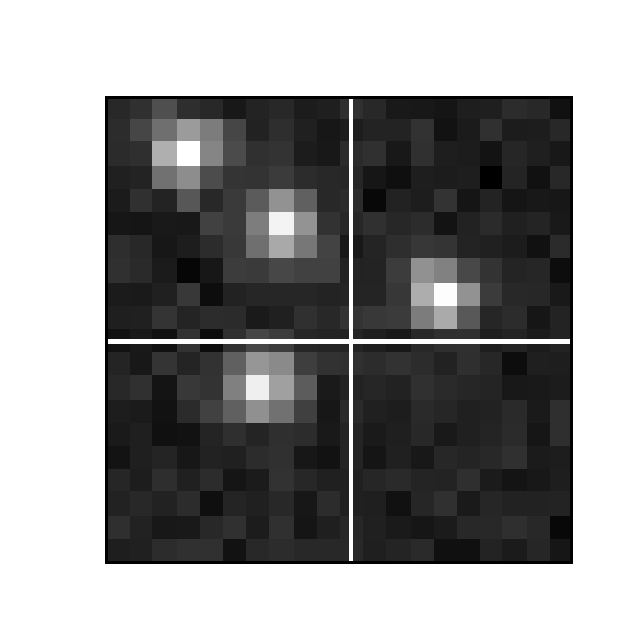
\includegraphics[width = 0.25\textwidth]{figures_vg/vi_figures/example_tiled_10.eps}
    \caption{Tiling a $20 \times 20$ pixel image into four $10 \times 10$ tiles.}
    \label{fig:ex_tiles}
\end{figure}

To make optimization tractable, the family $\mathcal{Q}$ is normally restricted to probability distributions
without conditional dependencies between some latent variables. In the most extreme case, known as mean-field variational inference, the variational distribution completely factorizes across all latent variables.

Our factorization has a spatial structure.
First, we partition the full $H \times W$-pixel image into disjoint $R \times R$-pixel tiles.
$R$ is chosen such that the probability of having three or more stars in one tile is small.
In this way, the cataloging problem decomposes to inferring only a few stars at a time (Section~\ref{sec:nn_architecture}).


Let $S = \sfrac{H}{R}$ and $T = \sfrac{W}{R}$ and assume without loss of generality that $H$ and $W$ are multiples of $R$.
For $s = 1, ..., S$ and $t = 1, ..., T$,
the tile $\tilde x_{st}$ is composed of the pixels
\begin{align}
    \tilde x_{st} = \{x_{hw} : Rs \leq h < R(s+1) \text{ and } Rt \leq w < R(t+1)\}.
    \label{eq:tiles}
\end{align}
Figure~\ref{fig:ex_tiles} gives an example with $R = 2$.

Let $\tilde N^{(s, t)}$ be the number of stars in tile $(s,t)$.
Because $\tilde N^{(s, t)}$ is random,
the cardinality of the set of locations and fluxes in each tile
is also random.
To handle the trans-dimensional parameter space,
we consider {\itshape triangular arrays} of latent variables
for each tile:
\begin{align}
    \tilde\ell^{(s, t)} &= (\tilde\ell_{N, i}^{(s, t)} : i = 1, ..., N; N = 1, 2, ...), \\
    \text{ and } \tilde f^{(s, t)} &= (\tilde f_{N, i}^{(s, t)} : i = 1, ..., N; N = 1, 2, ...),
\end{align}
where $\tilde\ell_{N, i}^{(s, t)}$ and $\tilde f_{N, i}^{(s, t)}$ are the elements of the triangular array corresponding to location and fluxes, respectively.
Tile locations $\tilde\ell_{N, i}^{(s, t)} \in [0, R]\times[0, R]$ give the location of stars within a tile. The fluxes $\tilde f_{N, i}^{(s, t)}$ are vectors in $\mathbb{R}^B_+$ (one flux for each band).

We refer to $(\tilde N^{(s, t)}, \tilde \ell^{(s, t)}, \tilde f^{(s, t)})_{s=1,t=1}^{S,T}$ as the {\itshape tile latent variables}. The distribution on tile latent variables factorize over image tiles:
\begin{align}
    \tilde q_\eta\big( \big(\tilde N^{(s, t)}, \tilde \ell^{(s, t)}, \tilde f^{(s, t)}\big)_{s=1, t = 1}^{S, T} \mid x\big)
    &=
    \prod_{s = 1}^S \prod_{t=1}^T
    \tilde q_\eta\big(\tilde N^{(s, t)}, \tilde \ell^{(s, t)}, \tilde f^{(s, t)} \mid x\big).
    \label{eq:factorize_patches}
\end{align}

We denote tile latent variables as $\tilde z$.
The ultimate latent variable of interest is $z = \{N, (\ell_i, f_{i,1}, ..., f_{i,B})_{i = 1}^N\}$, the catalog for the full image.
There is a mapping from $\tilde z$ to $z$.
First, the number of stars in the full catalog is given by the sum of the stars in each tile, $N = \sum_{s,t} \tilde N^{(s, t)}$.
Then, for every tile $(s,t)$, we index into the $\tilde N^{(s,t)}$-th row of the triangular array of tile latent variables $\tilde f^{(s,t)}$ and $\tilde \ell^{(s,t)}$.
The union of these fluxes and locations over all tiles form the full catalog (tile locations are shifted by the position of the tile in the full image to obtain locations in the full image).
See Figure~\ref{fig:tile_to_full_schm} for a schematic.


% \begin{align}
%     \{f_i\}_{i=1}^N = \Big\{\tilde f_{\tilde N^{(s, t)}, i}^{(s, t)} : i = 1, ..., \tilde N^{(s, t)}, s = 1, ..., S, t = 1, ..., T \Big\},
% \end{align}
% and the corresponding locations are
% \begin{align}
%     \{\ell_i\}_{i = 1}^N = \left\{\tilde \ell_{N^{(s, t)}, i}^{(s, t)} +
%     \begin{pmatrix}
%     Rs \\ Rt
%     \end{pmatrix}
%     : i = 1, ..., N^{(s, t)}, s = 1, ..., S, t = 1, ..., T\right\}.
% \end{align}
% The tile location is shifted by $(Rs, Rt)$ to obtain the location in the full image.

% Given this mapping from tile latent variables to the catalog of interest,
% \begin{align}
%  \big(\tilde N^{(s, t)}, \tilde \ell^{(s, t)}, \tilde f^{(s, t)}\big)_{s=1, t = 1}^{S, T}
% \mapsto
% \{N, (\ell_i, f_{i,1}, ..., f_{i,B})_{i = 1}^N\},
% \label{eq:patch_to_full_map}
% \end{align}
% a distribution on the tile latent variables induces a distribution on catalogs.

% Within each tile $(s,t)$, the distribution also fully factorizes:
% \begin{align}
%     \tilde q_\eta\big(\tilde N^{(s, t)}, \tilde \ell^{(s, t)}, \tilde f^{(s, t)} \mid x\big)
%     &=
%     \tilde q_\eta\big(\tilde N^{(s, t)} \mid x\big)
%     \prod_{n = 1}^\infty \prod_{i = 1}^n
%     \tilde q_\eta\big(\tilde \ell_{n,i}^{(s, t)} \mid x\big)
%     \tilde q_\eta\big(\tilde f_{n,i}^{(s, t)} \mid x\big).
%     \label{eq:factorize_within_patch}
% \end{align}

If $\tau$ is the mapping from $\tilde z$ to $z$,
then the variational distribution on catalogs $z$ is
\begin{align}
    q_\eta(z \mid x) := \tilde q_\eta(\tau^{-1}(z) \mid x),
    \label{eq:pull_back_of_q}
\end{align}
where $\tau^{-1}(z)$ is the pre-image of $z$ under $\tau$.
See Appendix~\ref{sec:eval_var_distr} for details on evaluating $q_\eta(z \mid x)$ for any given catalog $z$, which by \eqref{eq:pull_back_of_q} requires finding the pre-image $\tau^{-1}(z)$.


% for the figure
% {\color{blue} \tilde N^{(1,1)} = 2}

% \\

% \\

% \begin{pmatrix}
% (\tilde \ell, \tilde f)_{1, 1} & \\
% \color{blue} (\tilde \ell, \tilde f)_{2, 1} &
% \color{blue} (\tilde \ell, \tilde f)_{2, 2} &
% \end{pmatrix}^{(1,1)}

% \{{\color{Blue} N = 4},
% {\color{red} (\tilde \ell, \tilde f)^{(1,1)}_{2,1},
% (\tilde \ell, \tilde f)^{(1,1)}_{2,2}},
% {\color{DarkGreen} (\tilde \ell, \tilde f)^{(1,2)}_{1, 1}},
% {\color{Orange} (\tilde \ell, \tilde f)^{(2,1)}_{1, 1}}
% \}

\begin{figure}[tb]
    \centering
    \includegraphics[width = 0.9\textwidth]{figures/vi_figures/tile_to_full_schematic.png}
    %\vspace{-0.6cm}
    \caption{An example image with four tiles and four stars illustrating the relationship between the tile latent variables and the full-image catalog.
    To construct the full-image catalog, we index into the appropriate row of the triangular array for each tile.}
    \label{fig:tile_to_full_schm}
\end{figure}


\subsection{Variational distributions on image tiles}
\label{sec:distr_on_tiles}
We describe the variational distribution for each tile,
$\tilde q_\eta\big(\tilde N^{(s, t)}, \tilde \ell^{(s, t)}, \tilde f^{(s, t)} \mid x\big)$.
The latent variables fully factorize within each tile.
Dropping the index
$(s,t)$ in this subsection,
\begin{align}
    \tilde N &\sim \text{Categorical}(
    \omega; 0, ..., N_{max});  \label{eq:var_distr_n}\\
	\tilde \ell_{j, i} / R &\sim \text{LogitNormal}(\mu_{\ell_{j, i}}, \text{diag}(\nu_{\ell_{j, i}}) )\label{eq:var_distr_loc}; \\
	\tilde f^b_{j, i} &\sim \text{LogNormal}(\mu_{f^b_{j, i}}, \sigma^2_{f^b_{j, i}}), \label{eq:var_distr_f}
\end{align}
independently for $i = 1, ..., j$; $j = 1, ..., N_{max}$.
Here $\omega$ is a $(\tilde N_{max} + 1)$-dimensional vector on the simplex. $\mu_{\ell_{j, i}}$ and $\nu_{\ell_{j, }}$ are two-dimensional vectors---the covariance on locations is diagonal.
Note that in the exact posterior, $\tilde N$ has support on the nonnegative integers, whereas in the variational distribution $\tilde N$ is truncated at some large $N_{max}$.


These distributions were taken to match the constraints of the latent variables: fluxes are positive and right skewed, suggesting a log-normal; locations are between zero and $R$, suggesting a scaled logit-normal.

\subsection{Neural network architecture}
\label{sec:nn_architecture}

In each tile, the distributional parameters in \eqref{eq:var_distr_n},
\eqref{eq:var_distr_loc}, and \eqref{eq:var_distr_f} are the output of a neural network.
The input to the neural network is an $R \times R$ tile, padded with surrounding pixels.
Padding enables the neural network to produce better predictions inside the tile.
For example, a bright source outside but in the vicinity of the tile affects the pixel values inside the tile.
Padding the tiles allows the neural network access to this information.
Thus, while the distribution on tile latent variables factorize over tiles, the neural network is able to use information from neighboring tiles in producing the distributional parameters.

The appropriate amount of padding will depend on the PSF width in the analyzed image.
To catalog the crowded starfield M2 (Section~\ref{sec:results_on_m2}),
we set $R = 2$ and padded the tile with a three-pixel-wide boundary.
In cataloging a DECam image, we use larger tiles with more padding because the width of the PSF is larger in these images. There, we set $R = 10$ and used a five-pixel-wide boundary.


% Let $\hat x^{(s,t)}$ denote the padded tile pixel intensities (which includes all $B$ bands) and $h_\eta$ be the neural network.
% which returns the collection of distributional parameters %in~\eqref{eq:var_distr_n}-\eqref{eq:var_distr_f} on tile $(s,t)$.
% \begin{align}
%     h_\eta(\hat x^{(s,t)}) = (\omega^{(s,t)}, \mu_\ell^{(s,t)}, \nu_{\ell}^{(s,t)}, \mu_f^{(s,t)}, \sigma^{(s,t)}_f).
%     \label{eq:nn_output}
% \end{align}
% The same neural network is evaluated for all tiles $(s,t)$.
In amortized inference, the variational parameters $\eta$ are neural network weights.
The architecture consists of a convolutional layer followed by several residual network layers, which themselves contain convolutions, before ending with several fully connected layers (Figure~\ref{fig:starnet_arch}).
This architecture has been successful on image classification challenges such as ImageNet~\citep{imagenet2015}.
We tuned the architecture using Optuna, an automatic hyper-parameter optimization package \citep{optuna_2019}. 
Our search included the number of convolution layers, 
the number of fully connected layers,
the number of channels in the convolution layers, and the size of the fully connected layers. 

An input to the network is a padded tile, which consists of $B$ color bands. 
We also append an additional ``band" to the input, which 
is a one-hot encoding with
ones for pixels inside the tile, and zeros outside. 
We do this because the network is only responsible for inferring sources inside each tile, and this additional band gives
the network access to a feature which encodes the tile interior. 

See Appendix~\ref{sec:supp_nn_architecture} for further details 
concerning the parameters of our neural network architecture. 
% our focus in this paper is the application of neural networks to provide a variational posterior for cataloging starfields, not the network architecture per se.


% Convolutional layers are useful for localizing stars, as they make the network invariant to shifts in stellar location. The convolutional kernel in the first layer is $3\times3$ pixels, roughly the full width at half maximum (FWHM) of the PSF.

\begin{figure}[!tb]
    \centering
    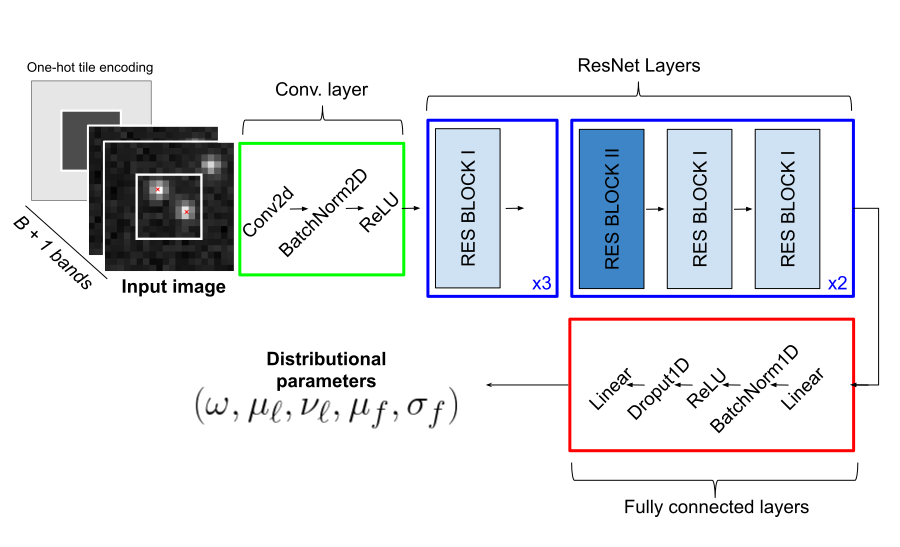
\includegraphics[width=\textwidth]{figures_vg/starnet_archetecture9.png}
%    \vspace{-1.cm}
    \caption{The neural network architecture. The DECam input is a two-band $20\times 20$ padded tile, 
    and the network returns distributional parameters corresponding to sources located in the $10\times 10$ tile outlined in white.
    In this example, there are two sources located in the $10\times10$ tile.
    The additional input band is a one-hot encoding with ones for pixels inside the tile, and zeros outside. 
    For further details concerning the residual network blocks (in blue), see 
    Appendix~\ref{sec:supp_nn_architecture}.
    }
    \label{fig:starnet_arch}
\end{figure}

% Note the output dimension of the neural network. For each tile $(s,t)$, the categorical parameter $\omega^{(s,t)}$
% lies on the simplex and has dimension $N_{max} + 1$.
% Furthermore, each index of the triangular array
% $i = 1, ..., \tilde N^{(s,t)}$, $\tilde N^{(s,t)} = 1, ..., N_{max}$
% describes a star. The star has a mean and variance for each location coordinate, and a mean and variance for its flux in each band.
% Thus, for each star $(\tilde N^{(s,t)}, i)$,
% the neural network outputs $2 \times (B + 2)$ parameters.
% In total, the neural network has output dimension $(N_{max} + 1) + (B + 2) \times (N_{max}^2 + N_{max})$.

% Recall that locations on the
% full image $\ell_{N, i}$ are parameterized to be in $[0, H] \times [0, W]$.
% On the tiles, locations $\ell^{(k)}_{N, i}$ are parameterized to be in
% $[0, s] \times [0, s]$.

Note that the output dimension of the neural network is quadratic in $N_{max}$: the outputs are parameters for a triangular array consisting of $\frac{1}{2}(N_{max}^2 + N_{max})$ sources.
Factorizing the variational distribution spatially keeps the output dimension manageable.
While the full image may contain many stars
(on the images that we catalog, the number of stars is on the order of thousands),
we set $N_{max} = 3$ for each tile.
Thus, the network is responsible for inferring only a few stars at once---a much easier task than inferring all stars simultaneously.

We emphasize that while the variational distribution factorizes over tiles, our method does not break the inference problem for the full image into isolated subproblems.
The likelihood of the full image does not factorize over tiles. Light from a star within a tile spills over into neighboring tiles, so the likelihood should not and does not decouple across image tiles.


\subsection{Estimation of model parameters}
\label{sec:model_params}
The generative model from section~\ref{sec:gen_model} requires
the specification of a PSF and a sky background. 
For the subimage of M2 we examine, 
we take the background at pixel $(i, j)$ to be an affine function in $i$ and $j$, so 
\begin{align}
    I_{ij}^{b} = \beta_0^{b} + \beta_1^{b} \times i + \beta_2^{b} \times j
\end{align}
where $(\beta_0^{b}, \beta_1^{b}, \beta_2^{b})$ are model parameters to be estimated, and 
vary by band $b$. 


We model the PSF as a weighted average between a Gaussian ``core" and a power-law ``wing" as described in~\cite{Xin2018psf}. For a given band, the PSF is modeled as 
\begin{align}
    \mathcal{P}(x, y) = \frac{\exp(\frac{-r^2}{2\sigma_1^2}) + 
                            b \exp(\frac{-r^2}{2\sigma_2^2}) + 
                            p_0(1 + \frac{r^2}{\beta\sigma^2_P})^{-\beta/2} }{1 + b + p_0},
\end{align}
where $r^2 = x^2 + y^2$. Though not explicit here, we allow the model parameters 
$(\sigma_1^2, \sigma_2^2, \sigma_P^2, \beta, p_0)$ to vary by band as well. 

We concatenate all model parameters into a real-valued vector $\phi$.
\jeff{You've been saying ``we'' a lot. Not that ``we'' needs to be avoided entirely. Or that you need start using the passive voice. But some of the time, there's a more concise way to say it by excluding us, the authors, from the sentence. Above, you might say something like ``let $\phi$ refer to all the model parameters collectively.''}
\jeff{It's probably better to explicitly list the model parameters though when you're defining $\phi$.}
\jeff{It's pretty unusual to use $\phi$ for model parameters, rather than $\theta$. Unless there's a reason, better to use $\theta$. It will be much easier on the reader, leaving them with more attention to devote to understanding the substantive ideas in the paper.
}
Our likelihood, and therefore posterior, now depend on $\phi$. We denote this dependence with a subscript, $\Prob_\phi$. 

We can simultaneously find an approximate posterior and 
estimate model parameters by jointly optimizing 
\begin{align}
(\eta^*, \phi^*) = \argmin_{\phi, \eta} \; \mathrm{KL}\big (q_{\eta}(N, \ell, f |X) \| P_{\phi}(N, \ell, f | X)\big)\label{eq:em_obj}
\end{align}
Variational EM~\cite{Jordan_intro_vi, neal2000varem, Beal2002varem} optimizes this objective with block coordinate descent on $\eta$ and $\phi$. Explicitly, 
\begin{align}
    \text{{\bf E-step: }} & 
    \eta_{t} = \argmin_\eta \; \mathrm{KL}\big (q_{\eta    }(N, \ell, f |X) \| \Prob_{\phi_{t - 1}}(N, \ell, f | X)\big)
    \label{eq:e_step}
    \\
    \text{{\bf M-step: }} & \phi_{t} = \argmin_{\phi} \; \mathrm{KL}\big (q_{\eta_t}(N, \ell, f |X) \| \Prob_{\phi}(N, \ell, f | X)\big), 
    \label{eq:m_step}
\end{align}
for iterations $t = 1, ..., T$. 

The E-step objective is exactly same as the KL objective in variational inference, equation~\ref{eq:kl_objective}, for fixed model parameters $\phi$. 
In other words, for fixed model parameters $\phi$, we are seeking the variational distribution closest the the true posterior under $\phi$. 

Recall that minimizing the KL divergence is equivalent to maximizing the ELBO (equation~\eqref{eq:elbo}). We can thus rewrite the M-step as 
\begin{align}
    \text{{\bf M-step: }} \phi_{t} &= \argmax_{\phi} \; \Expect_{q_{\eta}(N, \ell, f | X)}\Big[\log \Prob_\phi(X, N, \ell, f) - \log q_\eta(N, \ell, f)\Big] \\
    &= \argmax_{\phi} \; \Expect_{q_{\eta}(N, \ell, f | X)}\Big[\log \Prob_\phi(X, N, \ell, f)\Big]    \label{eq:m_step}
\end{align} 
To estimate model parameters, the goal is to optimize the marginal log-likelihood $\log \Prob_\phi(X)$; however, since $\log \Prob_\phi(X)$ is intractable, we optimize a lower bound as a surrogate for $\log \Prob_\phi(X)$. 

% \subsection{Estimation of the catalogue}
% In previous work \cite{Brewer_2013, Portillo_2017, Feder_2019}, the posterior on
% the latent variables $(N, \ell, f, c)$ was approximated using MCMC. In \cite{Portillo_2017, Feder_2019},
% a method was proposed to further reduce the posterior samples to a single point estimate
% which they call a {\itshape condensed catalogue}.
%
% While MCMC allows for the careful quantification of uncertainties, its computational cost
% is prohibitively large for large scale astronomical surveys. One possible alternative
% is to characterize the posterior using the maximum a posteriori estimate. Using the
% generative model from section~\ref{sec:gen_model}, the joint loglikelihood is
% \begin{align}
%   \log \mathcal{L}(N, \ell, f,& c) \stackrel{c}{=} \overbrace{\sum_{b = 1}^B \sum_{w = 1}^W \sum_{h = 1}^H
%         \Big\{-\frac{1}{2}\log{\lambda_{hw}^b} - \frac{(x_{hw}^b - \lambda_{hw}^b)^2}{2\lambda_{hw}^b}\Big\}}^
%         \text{Gaussian likelihood} + ...\notag\\
%         & ... + \underbrace{N\log(\mu HW) + \log N!}_\text{Poisson prior on $N$} -
%         \underbrace{\sum_{i = 1}^N (\alpha + 1)\log f_{N, i}^b}_\text{Pareto prior on fluxes} +
%         \underbrace{\sum_{b = 1}^B \sum_{i = 1}^N \frac{(c_{N, i}^b - \mu_c)^2}{2\sigma_c^2}}_\text{Gaussian prior on color}
% \end{align}
%
% To maximize this joint-loglikelihood, we must optimize over a discrete random variable $N$,
% so the usual gradient-based optimization methods do not apply. Indeed, it would require
% optimizing the locations, fluxes, and colors for each $N$ independently, and comparing
% the resulting log-likelihoods across $N$.
%
% We propose a method to approximate the maximum a posteriori estimate. Let
% $f:x \mapsto (\hat N, \hat \ell)$ be the function that maps data $x$ to the MAP estimates of
% the $N$ and $\ell$. In our procedure, we first train a neural network $q$ to approximate $f$.
% Thus, obtaining estimates for $N$ and $\ell$ at inference time is a computationally efficient
% forward pass through a neural network. With estimates in hand for $N$ and $\ell$,
% optimizing for $f$ can be done quickly with a few (quasi)-Newton steps; recalling
% our model for the photoelctron counts, equation~\eqref{eq:expected_intensity}, we see that
% are are simply regressing the observed image onto a linear combination of PSFs,
% and the coefficients of this linear combination are the desired fluxes.


\subsection{Wake-sleep training}
\label{sec:wake_sleep}
In mean-field variational inference, the E-step in equation~\eqref{eq:e_step} is often optimized by coordinate descent in the parameters of the variational distribution. 
The coordinate descent updates can be derived in closed form in the special case of exponential family models that are conditionally conjugate~\cite{Blei_2017_vi_review}. 

In our setting of amortized variational inference, stochastic 
optimization procedures have been employed with modern 
auto-differentiation tools to avoid the need for deriving 
analytic updates. Examples include black-box variational inference (BBVI)~\cite{ranganath2013black} 
and automatic-differentiation variational inference (ADVI)~\cite{kucukelbir2016automatic}. The latter 
is closely related to the reparameterization trick that \cite{kingma2013autoencoding, rezende2014stochastic} proposed to train deep generative models using the KL objective. 
These approaches all sample latent variables from $q_\eta$ and produce an unbiased estimate 
for the gradient of the KL; the optimization is done with stochastic gradient descent. 

However, the reparameterization trick does not apply when a latent variable is discrete, in our case, the number of stars $N$. Alternatively, the REINFORCE estimator~\cite{Williams1992reinforce}, which BBVI adapts, produces an unbiased stochastic gradient for both continuous and discrete latent variables. However, it often suffers from high variance in practice and the resulting stochastic optimization is slow. 

Stochastic gradients are difficult to compute in the E-step because the integrating distribution depends on the optimization parameter, $\eta$. 
The wake-sleep algorithm, originally proposed by~\cite{Hinton1995wake_sleep}, replaces the 
E-step objective with 
\begin{align}
    \argmin_{\eta} \Expect_{\tilde X \sim \Prob(\tilde X)}\Big[\KL(\Prob_\phi(N, \ell, f | \tilde X) \| q_\eta(N, \ell, f | \tilde X)\Big]
    \label{eq:sleep_obj}
\end{align}
called the {\itshape sleep phase}. We will see in section~\ref{sec:sleep_details} that a simple gradient estimator can be derived for the sleep phase objective, without 
reparameterization or REINFORCE. 

We comment on two key differences between the sleep objective and the E-step (equation~\eqref{eq:e_step}). First note the difference in ordering of arguments to the $\KL$. 
While optimizing $\KL(q\|p)$ in equation~\eqref{eq:e_step} does not depend on the intractable 
data likelihood $\Prob_\phi(X)$, the $\KL$ with arguments reversed does. 
As will be detailed in section~\ref{sec:sleep_details}, the outer expectation over the data makes this optimization objective tractable with various desirable properties. 
\jeff{Good to be more specific about the desirable properties}

The expectation over the data also gives different meaning to the sleep objective. The E-step objective seeks $\eta$ to minimize the $\KL$ between $P_\phi(N, \ell, f | X)$ and $q_\eta(N, \ell, f | X)$ {\itshape for fixed, observed data $X$},
in this case the $H\times W$ image. In contrast, the sleep objective seeks to minimize the $\KL$ {\itshape averaged over all possible data. } In other words, the target is no longer an approximate posterior for observed data, but rather an approximate posterior that is ``good on average" over possible data .

Moreover, ``possible data" is defined under our generative model from section~\ref{sec:gen_model}. In order for $q_\eta(N, \ell, f | X)$ to be a good approximation to
the true posterior when $X$ is observed data, then it is imperative that our generative model $\Prob_\phi(X)$ well-approximates the true underlying data-generating mechanism. 

Therefore, a {\itshape wake phase} is employed to tune the model parameters. The wake-phase objective is
\begin{align}
    \phi_{t} = \argmax_{\phi} \; \Expect_{q_{\eta}(N, \ell, f | X)}\Big[\log \Prob_\phi(X, N, \ell, f)\Big], 
    \label{eq:wake_elbo}
\end{align}
which is equivalent to the M-step in variational EM (equation~\ref{eq:m_step}). 

Note that stochastic gradients are easy to compute in the wake phase (M-step). Because the integrating distribution does not depend on the optimization parameter $\phi$ in the wake phase, unbiased stochastic gradients are computed simply as 
\begin{align}
    \nabla_\phi \log\Prob_\phi(X, N, \ell, f) \quad \text{ for } (N, \ell, f)\sim q_\eta
    \label{eq:mstep_grad}
\end{align}
While the E-step is not conducive to simple gradient estimators, we will see in section~\ref{sec:sleep_details} that our sleep-phase objective
results in a similarly straightforward gradient estimator as in equation~\eqref{eq:mstep_grad}. However,
we note that a consequence of replacing the E-step with the sleep phase is that the wake-sleep algorithm no longer targets a singular objective like that of equation~\eqref{eq:em_obj}. 

% Equation~\eqref{eq:wake_elbo} is equivalent to maximizing the ELBO in equation~\eqref{eq:elbo} with respect to model parameters $\phi$. 
% Since maximizing the ELBO is equivalent to 
% minimizing the $\KL$, we can also express the wake-phase objective as 
% \begin{align}
%     \phi_{t} = \argmin_{\phi} \; \mathrm{KL}\Big[\,q_\eta(N, \ell, f | X)\, \| \,\Prob_\phi(N, \ell, f | X )\,\Big]. 
% \end{align}

% In summary, given an initial $\eta_0$, $\phi_0$, and data $X$,
% for $t = 1, ..., T$, the wake-sleep algorithm alternates between two objectives: 
% \begin{align}
%     \text{{\bf Sleep: }} & 
%     \eta_{t} = \argmin_\eta \; \Expect_{\Prob_{\phi_{t - 1}}(\tilde X)}\Big[\KL\big ( \Prob_{\phi_{t - 1}}(N, \ell, f | \tilde X)\| q_{\eta}(N, \ell, f |\tilde X)\big)\Big]
%     \label{eq:sleep_kl}\\
%     \text{{\bf Wake: }} & \phi_{t} =  \argmin_{\phi} \; \mathrm{KL}\Big[\,q_{\eta_t}(N, \ell, f | X)\, \| \,\Prob_\phi(N, \ell, f | X )\,\Big]. 
%     \label{eq:wake_kl}
% \end{align}
% In the sleep phase, we are simulating data from $\Prob_\phi$ (i.e. ``dreaming") in 
% order to construct an approximate posterior. In the wake phase, we reveal the observed data $X$ and optimize model parameters $\phi$ so that our data-generating process aligns as closely as possible with the true data. 

\subsubsection{Decomposing the sleep objective}
\label{sec:sleep_details}
In this section, we decompose the sleep-phase objective in equation~\eqref{eq:sleep_obj} to examine its properties. We take $\phi$ as fixed in this section, and drop the explicit dependence of $\Prob$ on $\phi$.

First, we show that the objective does not depend on the intractable term $\Prob(X)$. 
We write
\begin{align}
 \argmin_{\eta} \; & \mathbb{E}_{\tilde X \sim P(\tilde X)}\Big[ \mathrm{KL}(P(N, \ell, f | \tilde X) \| q_\eta(N, \ell, f | \tilde X)\Big] \\
  &=\argmin_{\eta} \; \mathbb E_{P(\tilde X)}\Big[\mathbb E_{P(N, \ell, f | \tilde X)}\Big(\log P(N, \ell, f | \tilde X) - \log q_\eta(N, \ell, f | \tilde X) \Big)\Big]\\
&=\argmin_{\eta} \; \mathbb E_{P(\tilde X)}\Big[\mathbb E_{P(N, \ell, f | \tilde X)}\Big( - \log q_\eta(N, \ell, f | \tilde X) \Big)\Big]\\
&=\argmin_{\eta} \; \mathbb E_{P(\tilde X, N, \ell, f)}\Big[- \log q_\eta(N, \ell, f | \tilde X) \Big]\label{eq:sleep_loss_simple}
\end{align}
Crucially, the integrating distribution is $P$, which does not depend on the optimization parameter $\eta$.
In the E-step of variational EM (equation~\eqref{eq:e_step}), the integrating distribution is $q_\eta$, resulting in the need for reparameterization or other adjustments to compute stochastic gradients. 
Here, unbiased stochastic gradients can be obtained simply as 
\begin{align}
    g = -\nabla_\eta \log q_\eta(N, \ell, f | \tilde X) \quad \text{ for } (N, \ell, f, \tilde X)\sim P
\end{align}

In other words, we simulate {\itshape complete} data $(N, \ell, f, \tilde X)$ from our generative model and evaluate the loss $-\log q_\eta(N, \ell, f | \tilde X)$. 
This loss encourages $q_{\eta}(N, \ell, f | \tilde X)$ to map images $\tilde X$ to a probability distribution with large mass on $(N, \ell, f)$.

We examine the loss $-\log q_\eta(N, \ell, f | \tilde X)$ more closely. Recall that $q_\eta$ factorizes over image patches. Having sampled latent variables and the $(N,\ell,f)$ and the $H\times W$ image $\tilde X$ from $P$, we convert the latent variables to their patch parameterization $(N^k, \ell^k, f^k)_{k = 1}^K$. 

For a given image patch, the latent variables $N^k$, $\ell^k$, $f^k$ also factorize in $q$, so 
\begin{align}
    - \log q_\eta(N^k, \ell^k, f^k | \tilde X) = 
        - \log q_\eta(N^k | \tilde X) 
        - \log q_\eta(\ell^k | \tilde X) 
        - \log q_\eta(f^k | \tilde X). 
        \label{eq:sleep_loss_decomp}
\end{align}
We examine each term separately. On patch $k$, the number of stars $N^k$ is categorical with parameter $\omega^k$. The loss function for the number of stars becomes
\begin{align}
    - \log q_\eta(N^k | \tilde X) = -\sum_{n = 0}^{N_{max}} 1\{N^k = n\} \log \omega^k_n, 
\end{align}
the usual cross-entropy loss for a multi-class classification problem. 

For the last two terms, recall that location coordinates are logit-normal and fluxes are log-normal. For a given index $(i, N)$ let $y^k_{i,N}$ generically denote either the 
logit-location or log-flux for that star, 
and let $\mu^k_{i,N}$ and $\sigma^{k}_{i,N}$ generically denote its variational parameters,
the mean and standard deviation of a Gaussian. Then the losses in the last two terms of equation~\ref{eq:sleep_loss_decomp} are of the form 
\begin{align}
    -\log q_\eta(y^k_{i,N} | \tilde X) = 
        \frac{1}{2(\sigma^{k}_{i,N})^2}(y^k_{i,N} - \mu^k_{i,N})^2
         + \log\sigma^{k}_{i,N}
         + \frac{1}{2}\log(2\pi)
\end{align}
We also give an interpretation: $y_{i,N}$ is the true, simulated latent variable (either logit-location or log-flux); $\mu^k_{i,N}$ is the predicted value for that latent variable of the neural network. $\sigma^{k}_{i,N}$ is also outputted by the neural network, representing uncertainty -- the second term encourages small uncertainties, but this is 
balanced by the scaling of the error $(y^k_{i,N} - \mu^k_{i,N})^2$ in the first term. 

In summary, the sleep-phase results in a supervised learning problem on complete data simulated from our generative model. 

\subsubsection{Reverse versus forward KL}
\label{sec:kl_q_p}
TODO: something about forward KL overestimates uncertainties, see figure~\ref{fig:kl_q_p_schematic}. 

\begin{figure}[!h]
    \centering
    \includegraphics[width = 0.5\textwidth]{figures/kl_q_p_schematic.png}
    \caption{A toy example where the true distribution is a bivariate Gaussian on 
    $\theta = (\theta_1, \theta_2)$ with positively correlated components. 
    $q$ is a mean-field variational approximation. Left, the optimal $q$ found 
    optimizing $\KL(q\|p)$; right, the optimal $q$ found optimizing $\KL(p\|q)$. }
    \label{fig:kl_q_p_schematic}
\end{figure}

% \begin{itemize}
%     \item Number of stars $N$ is {\color{red}{\bf categorical}} with parameter $\omega$. 
%     \item Locations $\ell_n$ are {\color{blue}{\bf logitnormal}} with parameters $\mu_{\ell, n}$ and $\nu_{\ell, n}$
%     \item Fluxes $f_n$ are {\color{orange}{\bf lognormal}} with parameters $\mu_{f, n}$ and $\sigma^2_{f, n}$. 
% \end{itemize}


\section{Related work}
\label{sec:related_work}
\subsection{Connection with variational EM}
% Wake sleep was originally proposed by~\cite{Hinton1995wake_sleep}, and revisited in~\cite{bornschein2014reweighted, le2018revisiting}. \cite{le2018revisiting} proposed wake-sleep as a viable alternative to the reparameterization trick when training discrete-distribution latent variable models. 

% We also note the connection between wake-sleep and variational EM~\cite{Jordan_intro_vi, neal2000varem, Beal2002varem}. For iterations $t = 1, ..., T$, variational EM alternates between two objectives: 
% \begin{align}
%     \text{{\bf E-step: }} & 
%     \eta_{t} = \argmin_\eta \; \mathrm{KL}\big (q_{\eta    }(N, \ell, f |X) \| P_{\phi_{t - 1}}(N, \ell, f | X)\big)
%     \label{eq:e_step}
%     \\
%     \text{{\bf M-step: }} & \phi_{t} = \argmin_{\phi} \; \mathrm{KL}\big (q_{\eta_t}(N, \ell, f |X) \| P_{\phi}(N, \ell, f | X)\big)
%     \label{eq:m_step}
% \end{align}
% The M-step in variational EM and the wake phase in wake-sleep are the same (compare equations~\eqref{eq:wake_kl} and \eqref{eq:m_step}). 
% Variational EM can be viewed as coordinate descent on the KL, with each step alternating between updating $\eta$ and $\phi$. The overall objective is 
% \begin{align}
% (\eta^*, \phi^*) = \argmin_{\phi, \eta} \; \mathrm{KL}\big (q_{\eta}(N, \ell, f |X) \| P_{\phi}(N, \ell, f | X)\big)\label{eq:em_obj}
% \end{align}

% The sleep phase is analogous to the E-step (compare equation~\eqref{eq:sleep_kl} and \eqref{eq:e_step}). 
% The sleep phase objective reverses the arguments of the KL in the E-step so it becomes more amenable to stochastic gradient methods. However, wake-sleep is no longer optimizing a single objective as in equation~\ref{eq:em_obj}. 

% \subsection{Cataloging of stellar fields}
% TODO

SDSS has a default cataloger, PHOTO~\cite{lupton2001sdss}. It timed out on the crowded starfield that we examine, M2. 

DAOPHOT~\cite{stetson2987daophot} is an algorithmic routine designed for crowded starfields. To detect stars, the observed image is convolved with a Gaussian kernel. The convolved image is scanned for peaks above a given threshold, which are then labeled as stars. \cite{An_2008_m2} applied DAOPHOT to catalog M2, and we refer to this as the DAOPHOT catalog in our comparisons. 

\cite{Brewer_2013, Portillo_2017, Feder_2019} employed probabilistic cataloging, and inference was using MCMC. In the most recent work \cite{Feder_2019}, a runtime of 30min was reported to catalog a $100 \times 100$ subimage of M2. In the sequel, we will compare the catalog produced from their MCMC procedure against the catalog produced by our variational posterior. We will show that our method is several orders of magnitude faster at inference time. 

Our generative model is most similar to \cite{Portillo_2017, Feder_2019}, except they used an exponential prior on the number of stars instead of Poisson. 
In \cite{Brewer_2013}, a broken power-law prior was used for the flux, and further hyper-priors are placed on the parameters of the broken power-law. The parameters of the broken power-law are treated as latent variables. In our case, this would be analogous to placing a hyper-prior on $\alpha$ from equation~\eqref{eq:flux_prior}. 
Alternatively, though not explored in this work, we can treat our prior parameter as a model parameter and optimize them in the wake phase. The same principle applies to the Poisson prior parameter, $\mu$. 

Finally, \cite{Portillo_2017, Feder_2019} use the default SDSS estimates. As will be shown in the sequel, the default SDSS estimates for the PSF and background can be improved for a better model fit. $\cite{Brewer_2013}$ treats the PSF parameters as latent variables in their MCMC chain. In contrast, 
our we estimate model parameters in the wake phase. 

\section{Results}
\label{sec:results}

Section~\ref{sec:estep_sleep_compare} motivates the wake-sleep approach by comparing variational posteriors obtained by optimizing the ELBO against those obtained by optimizing the sleep objective. 
Then, StarNet is tested on blended simulated stars in Section~\ref{sec:deblending_test}. 
Finally, in Section~\ref{sec:results_on_m2}, StarNet is employed to catalog the SDSS image of the M2 globular cluster. The StarNet catalog is compared with existing cataloging methods. 

\subsection{ELBO versus sleep objective}
\label{sec:estep_sleep_compare}

This subsection compares the resulting variational posteriors obtained by optimizing the sleep objective~\eqref{eq:sleep_obj} 
against those obtained by optimizing the ELBO~\eqref{eq:elbo}.
A simple example demonstrates that there exist shallow optima in the ELBO where the variational posterior on locations does not concentrate around the true locations.
On this example, fitting the variational posterior using the sleep phase is able to avoid shallow optima. 
Because the data were simulated with known PSF and background, the wake phase is not needed. 

The simulated $20\times20$ single-band image $x_{test}$ is shown in Figure~\ref{fig:toy_example}.
The image has four stars, each with the same flux. It is partitioned into four $10\times 10$ tiles, which are the inputs to the neural network. 
The image was fixed for this experiment. 

\begin{figure}[!h]
    \centering
    \vspace{-1em}
    \includegraphics[width = 0.3\textwidth]{figures/vi_sleep_ex_figure.png}
    \vspace{-1.7em}
    \caption{Our $20\times 20$ pixel test image with four stars, partitioned into $10\times 10$ tiles. }
    \label{fig:toy_example}
\end{figure}

The generative model is set with the prior on the number of stars $N$ to have mean $\mu = 4$ and the prior on flux to have power law slope $\alpha = 0.5$. 
With these prior parameters, we compare directly optimizing the ELBO on the test image, 
\begin{align}
\mathcal{L}_{elbo}(\eta; x_{test}) = \Expect_{q_{\eta}(z | x_{test})}\Big[\log p(x_{test}, z) - \log q_{\eta}(z | x_{test})\Big],
\label{eq:elbo_on_test}
\end{align}
against optimizing the sleep objective $\mathcal{L}_{sleep}(\eta)$ in~\eqref{eq:sleep_obj}. Note that optimizing the sleep objective does not depend on $x_{test}$: the sleep phase only requires sampling catalogs from the aforementioned prior and simulated images conditional on each catalog. 

Figure~\ref{fig:optim_path} charts the ELBO~\eqref{eq:elbo_on_test} as the optimization proceeds.
In the first approach (Figure~\ref{fig:optim_path}a), the ELBO was optimized with stochastic gradient descent and the REINFORCE estimator.
This optimization did not converge, likely due to the high variance of the REINFORCE estimator. 
For a lower variance gradient estimator, the second approach (Figure~\ref{fig:optim_path}b) employed the reparameterized gradient.  To employ this gradient estimator, we analytically integrated the ELBO with respect to the number of stars $N$ to remove the discrete random variable. 
See Appendix~\ref{sec:reparam_details} for details about the gradient estimators. 
The lower variance of the reparameterized gradients allowed the optimization to converge to stationary points. 
However, depending on the initialization, the variational distribution converged to points where the ELBO is non-optimal (e.g. restarts 3 and 6). 

In contrast, Figure~\ref{fig:optim_path}c shows the ELBO as the sleep phase proceeds. 
While the sleep phase does not directly optimize the ELBO, the ELBO increases nonetheless as the variational posterior better approximates the true posterior. 
Optimizing the sleep objective consistently converged to a similar ELBO across all restarts and appeared to avoid the shallow local optimum found in Figure~\ref{fig:optim_path}b.

The bottom row of Figure~\ref{fig:optim_path} displays the estimated locations, given by the mode of the fitted variational distribution. 
The bottom left shows these locations after getting stuck in a local minimum. 
In the tile with two stars, both estimated locations were placed on one star. 
For correct detections, one of the locations should be placed on the second star. 
However, to move one location to the second star, the optimization path must traverse a region where the log-likelihood is lower than the current configuration. 
The displayed configuration is a local optima where the gradient with respect to its locations is approximately zero.
In contrast, the sleep phase optimization consistently placed its mode around the four true stars. 
An example of correct detections after sleep phase optimization is shown in the bottom right of~Figure~\ref{fig:optim_path}.

\begin{figure}[!htb]
    \centering
    \begin{subfigure}[t]{0.9\textwidth}
    \centering
    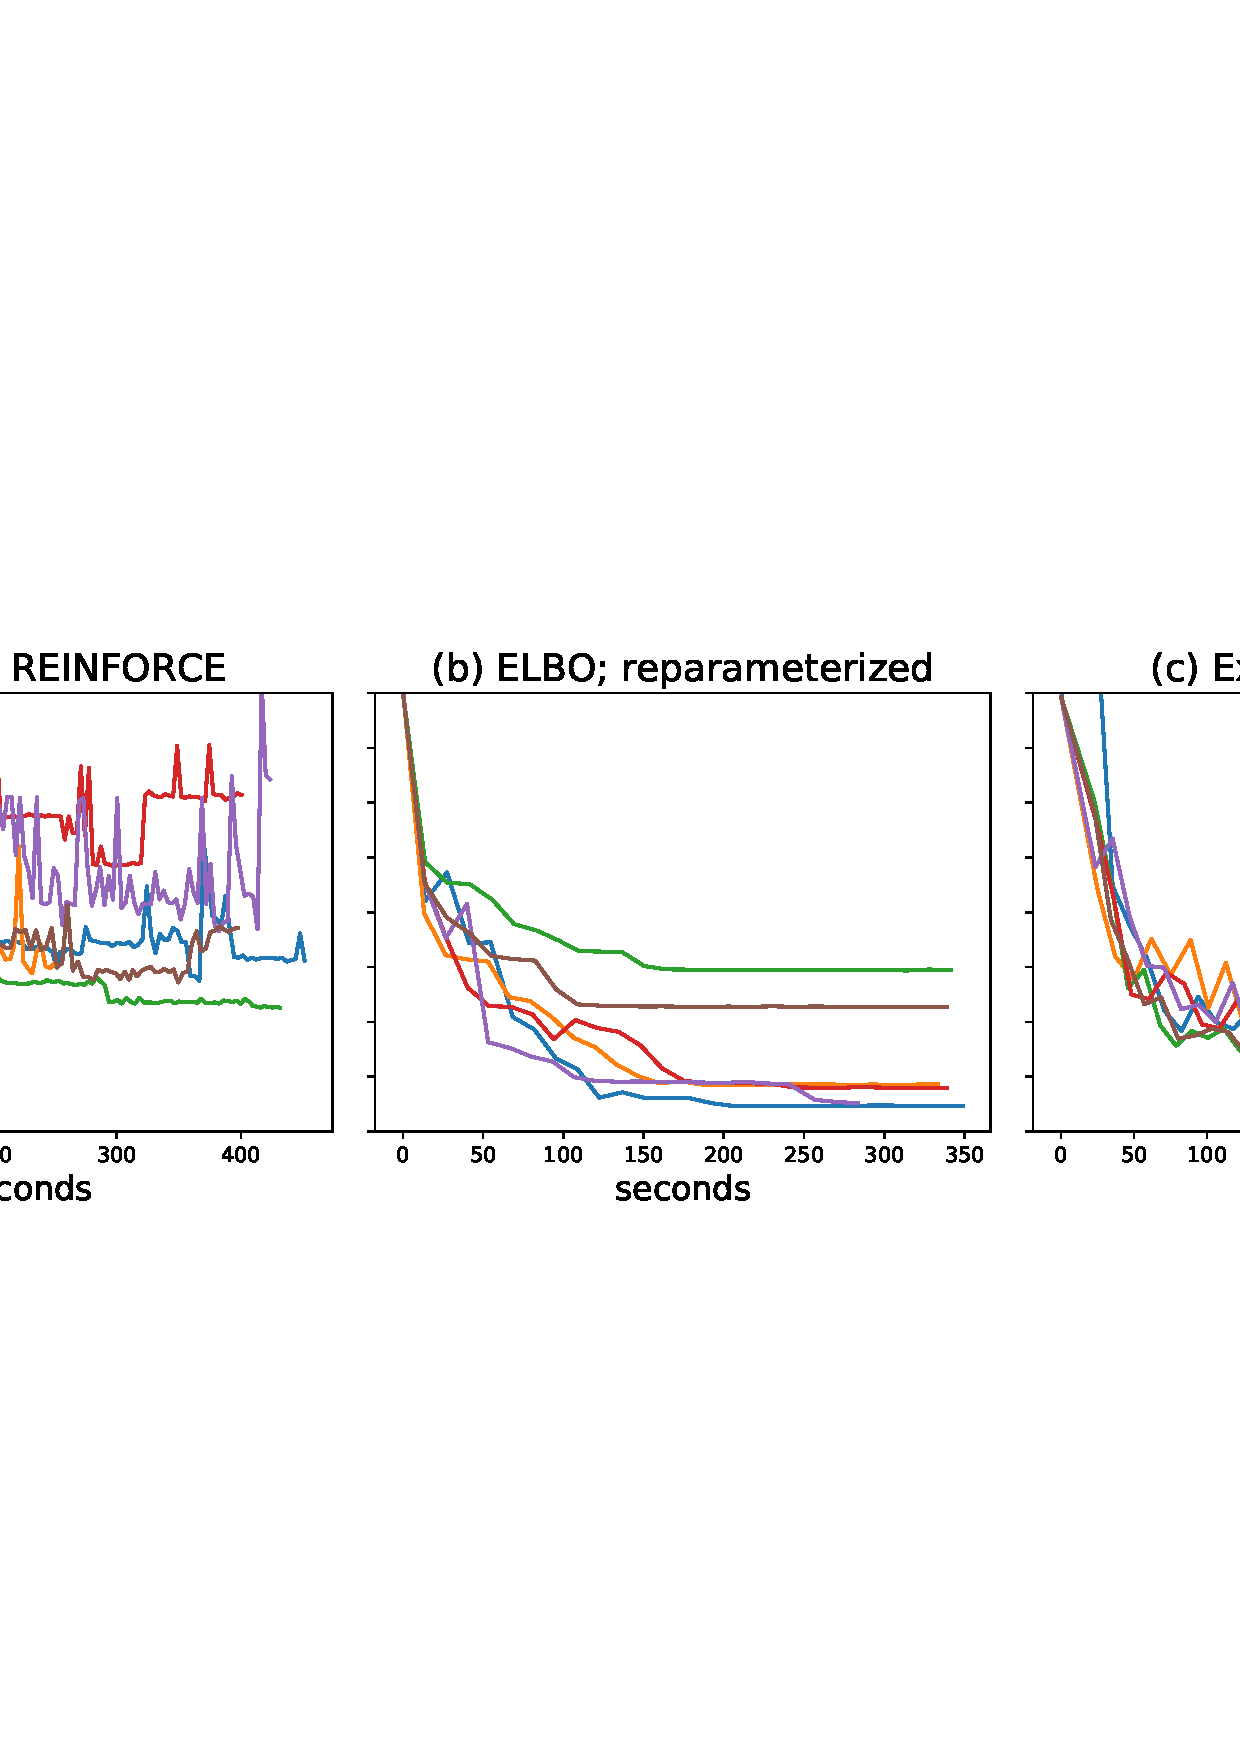
\includegraphics[width=\textwidth]{figures/optim_path_compare.png}
    \end{subfigure}
    \begin{subfigure}[t]{\textwidth}
    \centering
    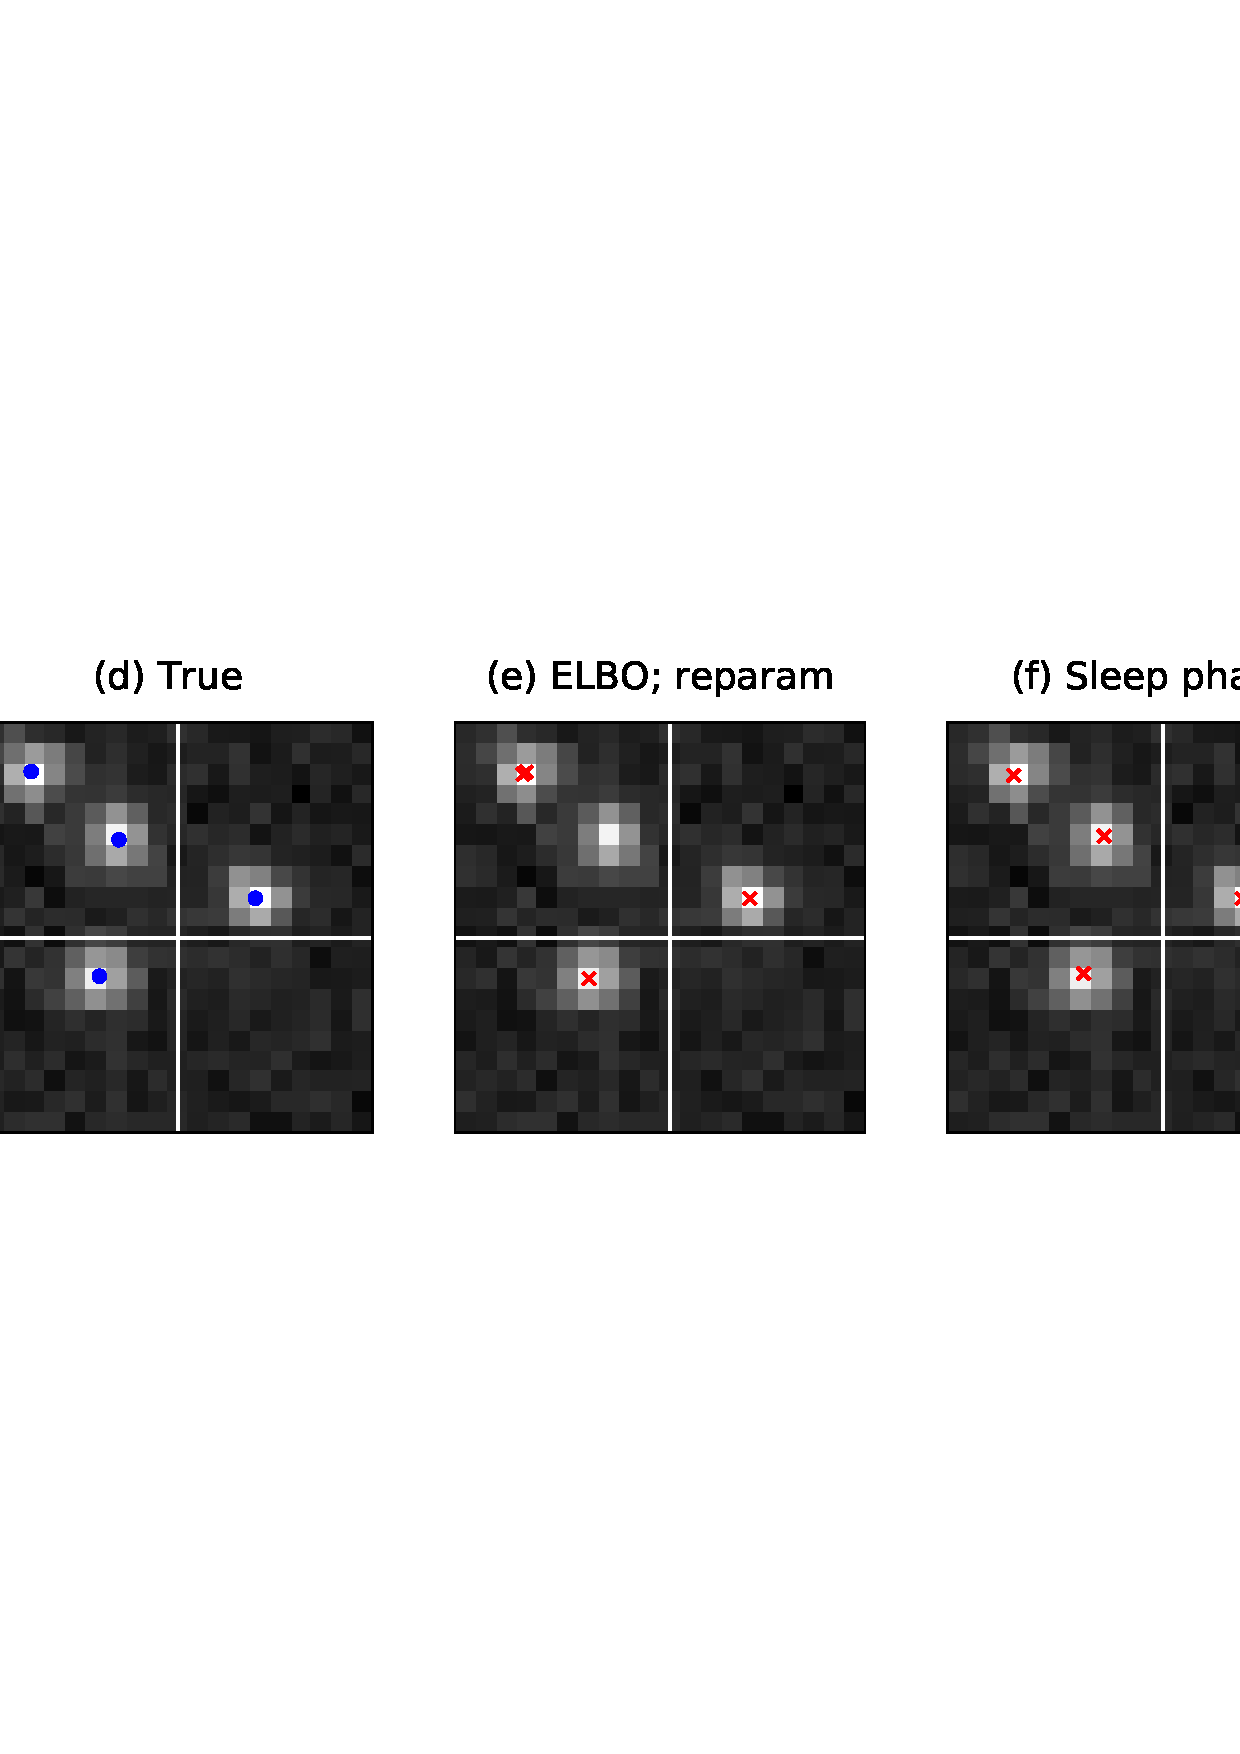
\includegraphics[width=0.55\textwidth]{figures/optim_path_detect_compare.png}
    \end{subfigure}
    \vspace{-3em}
    \caption{(Top row) The ELBO as the optimization progresses 
    for six random restarts. 
    The bold pink line in all plots is the sleep phase ELBO path, averaged over six restarts. 
    (Bottom row) Estimated locations from two variational posteriors shown in red. On the left, an instance where optimizing the ELBO using the reparameterized gradient landed in a local optimum.
    On the right, an example of detections under 
    sleep-optimized variational posterior. }
    \label{fig:optim_path}
\end{figure}

Figure~\ref{fig:gradzero_cartoon} shows schematic of this general phenomenon. When the mean location under the variational posterior is far from the true location, the gradient of the ELBO with respect to location mean vanishes. 
Because the PSF is nearly zero everywhere except for a few pixels around each location, a small shift in location does not significantly change the likelihood unless the location mean is within a ``PSF radius" of the true location.
On the other hand, the sleep phase objective is quadratic in the location mean -- see~\eqref{eq:gaussian_sleep_loss}. Thus, the further the location mean from the true location, the larger the gradient. The gradient does not vanish in the sleep objective. 

\begin{figure}[!htb]
    \centering
    \includegraphics[width=\textwidth]{figures/gradzero_cartoon3.png}
    % \centering
    % \begin{subfigure}[t]{0.8\textwidth}
    % \centering
    % \includegraphics[width=\textwidth]{figures/gradzero_cartoon.png}
    % \end{subfigure}
    % \begin{subfigure}[t]{\textwidth}
    % \centering
    % \includegraphics[width=0.55\textwidth]{figures/gradzero_cartoon2.png}
    % \end{subfigure}
    % \vspace{-3em}
    \caption{An illustration of vanishing gradients when the location mean under the variational distribution (red) is far from the true location(blue). 
    For large delta, the the ELBO objective is flat, 
    and hence gradients with respect to location is nearly zero. 
    In contrast, the sleep objective is quadratic in the location mean, and the gradient does not vanish. }
    \label{fig:gradzero_cartoon}
\end{figure}

Also note that low-variance gradients of the ELBO were constructed by analytically integrating $N$ in the objective, so the reparameterization trick could be applied. 
In this example, $N_{max} = 2$ so the neural network infers either 0, 1, or 2 stars on each tile. 
Since the variational distribution factorizes over the four tiles, integrating $N$ is a summation of $3^4 = 81$ terms.
On larger images with more tiles, analytically integrating $N$ would be computationally infeasible, and REINFORCE gradients would be required. 

To illustrate on a larger example, Figure~\ref{fig:sim_data100x100} displays our results on a simulated $100\times 100$ image with fifty stars. The tiles again consisted of $10\times 10$ pixels. Optimizing the sleep phase objective resulted in near perfect in estimation of locations; optimizing the ELBO appears to be hindered by regions with little gradient information and is slow to converge. 

\begin{figure}[!htb]
    \centering
    \begin{subfigure}[!t]{0.4\textwidth}
    \centering
    \includegraphics[width=\textwidth]{figures/optim_path_compare_100x100.png}
    \end{subfigure}
    \begin{subfigure}[!t]{0.59\textwidth}
    \centering
    \includegraphics[width=\textwidth]{figures/optim_path_detect_compare_100x100.png}
    \end{subfigure}
    \caption{(Left) The negative conditional log-likelihoood $p(x|\hat z)$, where $\hat z$ is the mode of the variational posterior. (Right) Detections on a $100\times 100$ image, with true locations in blue, and estimated locations in red. }
    \label{fig:sim_data100x100}
\end{figure}

\input{5b-results-m2}

% \section{Discussion}
% \label{sec:discussion}
% Probabilistic modeling provides a framework to 
produce catalogs with statistically principled uncertainties.
We defined a statistical model, and uncertainties are captured by a Bayesian posterior over the space of all catalogs.
In previous work on probabilistic cataloging, samples from the posterior were obtained using MCMC. 
While samples eventually converge to the exact posterior in theory, the computational cost of MCMC prohibits its application to large-scale astronomical surveys. 

Our method instead produces an approximate Bayesian posterior using amortized variational inference, which has potential to scale Bayesian inference to large astronomical surveys.
After a one time cost of training, the network efficiently returns approximate posteriors for batches of images.
The neural network is trained using the wake-sleep algorithm which optimizes an objective different than the ELBO used in traditional variational inference. 
In this problem of localizing stars, 
the ELBO suffers from shallow optimum. 
The wake-sleep algorithm produced approximate posteriors that were more reliably concentrated around the true catalogs. 
\jeff{This paper reads a lot like a narrative still. The term ``we'' shows up several hundred times, often unnecessarily, for example. (Perhaps one third of these occurrences could be safely eliminated by reworking sentences.) It's preferable to focus the reader on the model/results rather than on our experiences.
}
% \jeff{Wake-sleep didn't really avoid the minima---it optimized a different objective entirely.}

In addition to scalability, a key advantage our approach has over MCMC is the ability to estimate model parameters such as the PSF and sky background.
While the current work focuses on PSF models, our method can be extended to more general sources such as galaxies.
Each source would have an additional latent variable specifying whether it is a star or galaxy. If the source is a galaxy, it would have latent variables describing its shape in addition to its location, flux, and color variables. The statistical model would need to include likelihoods for galaxy sources in addition to the PSF model.

One promising direction is to also use neural networks in the wake phase and fit a deep generative model for galaxies~\cite{Regier2015ADG}. Here, a neural network encodes a conditional likelihood of galaxy images given source latent variables. Thus, neural networks would be trained in both the sleep and wake phase -- the sleep phase trains the approximate posterior while the wake phase trains the galaxy model. Using a neural network to encode a likelihood extends the flexibility of galaxy models beyond simple parametric forms. 

Going even further, models for artifacts such as cosmic rays and bleed trails~\cite{Desai_2016} could be estimated in this framework.
% \jeff{Readers likely won't know what cosmic rays and bleed trails are. Maybe cite something here that explains them, for the curious reader.}
These artifacts produce artificial bright spots in an image which do not correspond to celestial objects.
Currently, pixels corresponding to these objects need to be masked by a preprocessing routine before a catalog can be produced. 
However, including these artifacts in a statistical model allows for the quantification of uncertainties in their detection. 
Moreover, credible intervals for latent variables of interest can be computed by marginalizing out the uncertainties in artifact detection. 
In this way, the uncertainties in artifact detection can be propagated to uncertainties for variables of interest. 

Our ultimate goal is to provide a pipeline from raw images to catalogs to downstream analyses, where errors are appropriately quantified in each step. 
The size of the data in upcoming surveys is immense by any standard. 
Our method holds promise for scaling inference to meet the challenges of these future surveys. 
Our statistical framework lays the foundation for future work in building flexible models to incorporate the cataloging of all celestial objects. 

% provides a statistical framework for 


% Our method is scalable, works well on deblending, provides approximate inference in achieving this goal .... TODO. 

\jeff{I think there's a bibtex command like ``max\_names'' that will insert et al. You might want to cap the number of names at 6: some of these citations are really long.}
\jeff{A lot of the citations have letters in the wrong case. e.g. ``decam'' instead of ``DECam'', ``lsst'' instead of ``LSST'', ``markov'' instead of ``Markov'', ``Cmu'' instead of ``CMU'', etc.}
\jeff{Also some first names are spelled out in full while others are initials.}

\bibliographystyle{unsrt}
% \bibliographystyle{Chicago} doesn't work for some reason
\bibliography{bibliography}

\appendix
\section{Results on Stripe-82}
\input{A1-results-sparse_field}

\end{document}
